% chapter 5 conclusion and future work
\chapter{改进后的仿真实验结果与分析}

本章主要阐述对程序填空评测改进算法与初期算法的仿真实验的部署、运行结果
展示和结果分析。

\section{实验环境和参数设置}
\subsection{实验环境}
Linux 系统笔记本,安装 Node.js 服务器运行环境(运行本地服务端)。测试数据
库服务(服务器)、测试评测系统服务(服务器)。

\subsection{参数设置}
\begin{enumerate}
  \item 以图\ref{fig:prob_desc}的题目作为实验题目,从数据库提取考试中学生的提交作为实验样
本。
  \item 根据上章服务器对学生提交答案的处理算法,对实验样本的提交数据进行处理,批量提交评测请求到
  评测系统。评测完毕后,批量查询分数进行统计。
  \item 对比参照组为两组,分别为使用改进前评测算法(动态测试评测只提交一次程序评测)和改进后评测算法(每个填空答案对应一次评测)。
  \item 对比结果为两组算法得出的动态测试评测得分。
\end{enumerate}

\section{结果图表与具体分析}
图\ref{figdynamic_graph}与图\ref{fig:grade_graph}
为使用考试学生提交数据为实验样本的动态评测结果的结果折线图
和为同样的实验中动态测试评测算法改进前与改进后的总得分折线图。

\begin{figure}[h]
	\centering
	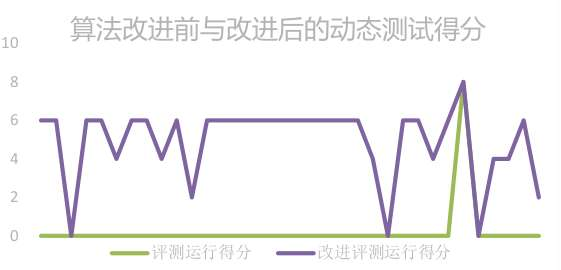
\includegraphics[width=0.5\textwidth]{image/chapter5/1}
  \caption{改进前与改进后的动态测试评测分数对比(横轴为学生,纵轴为得分,满分为8分)}
 	\label{fig:dymamic_graph}
\end{figure}

\begin{figure}[h]
	\centering
	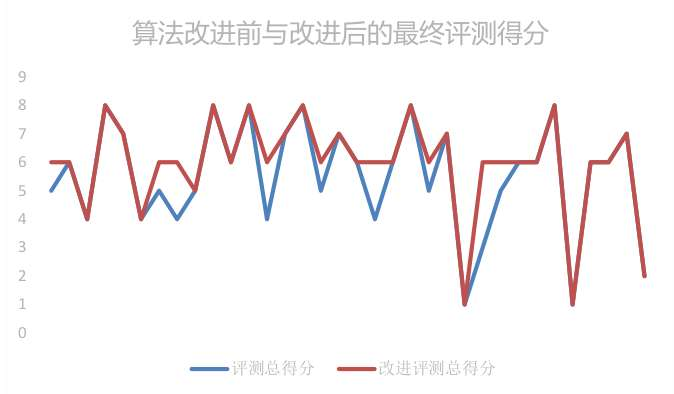
\includegraphics[width=0.5\textwidth]{image/chapter5/2}
	\caption{算法改进前与改进后的评测总得分}
 	\label{fig:grade_graph}
\end{figure}


\subsection{结果分析}
从动态测试评测的结果图表来看,动态测试的评测的评分变化幅度很大,许多原
本评分为0分的在改进算法后都有了较高的分数。这是除去第二空中const
声明缺失造成的整体的编译不通过的影响后的改进结果。将每个空的学生答案独立与其它标准答
案结合在一起进行评测,即使出现编译错误,也只会影响到出现语法错误的该空的分
值,不会影响到其它填空的评分。

而从最终得分的结果图表来看,动态测试部分评测分的提高带动提高了不少学生的
最终得分,使得最后的评分结果更为合理,动态测试也起到了应有的评分作用。

\clearpage
